\section{Report on Technical Progress}

\subsection{Framework for GPU processing}

In the early stages of the project it was decided that it would be necessary to create a custom application to process and display voxel data.
The rationale behind doing this instead of using an existing solution such as Matlab or Octave was threefold:

\begin{itemize}
	\item The sample dataset from the Southampton Gait Tunnel is stored in a custom binary format, the parsing and display of which is
		performed by an C library, Vis4D, written by Richard Seely.
		The library is efficient and well-tested, therefore it would be beneficial to make as much use of it as possible.
	\item One of the goals of the project is to investigate ways in which the algorithms can be made parallelizable and applicable to real-time processing.
		As a prototyping language Matlab is generally less suitable for real-time or high-performance computing than a lower-level language such as C.
	\item The key aspect of this area of research that sets it aside from others in the field is that it focuses on 3D datasets.
		Visualising this 3D data TODO
\end{itemize}

It was decided to create an application that would run image-processing and recognition algorithms on the GPU.
The algorithms would be 


Toolkits used, and why?

Design of application.  Stating that UML isn't really needed but here it is anyway.

Screenshots

\subsection{Computation of global position}\label{LocatingCenter}

The very first pre-processing step is to locate the center of the figure and to calculate some basic parameters such as the height.

\subsection{Cross-correlation}

The first attempt at locating a thigh in the 3D image used the mathematical cross-correlation operator.
A 3D ``thigh-filter'' was generated using Matlab which matched the shape and size of a typical thigh from the sample data.
This was then cross-correlated with the 3D voxel-space image to determine where in the image the thigh was most likely to be.

\bigskip
\noindent Cross-correlation is similar to convolution in that two signals are moved over each other to produce a third signal describing where they best match.
For 3-dimensional discrete input images $f$ and $g$, the cross-correlation image $(f \star g)$ is defined as:

\begin{equation}
	(f \star g)_{(\delta x,\delta y,\delta z)} = \sum_{x=1}^{s_{x}} \sum_{y=1}^{s_{y}} \sum_{z=1}^{s_{z}} f_{(x,y,z)} \cdot g_{(x+\delta x,y+\delta y, z+\delta z)}
\end{equation}

Where $s$ is the size in pixels of the image $f$.

In our case we are not interested in the translation $(\delta x,\delta y,\delta z)$ of the thigh-filter $f$ over the voxel-space image $g$, but rather its rotation.
It is assumed that the thigh has two degrees-of-rotation: $\theta$ - the rotation that makes the leg move in the walking direction, and $\alpha$ - any side-to-side movement of the leg.
We implement this by introducing a transformation matrix $\mathbf{M}(\alpha,\theta)$:

\begin{equation}
	\mathbf{M}(\alpha,\theta) =
	\left(\begin{array}{ccc}
		cos(\alpha) & 0 & sin(\alpha) \\
		0 & 1 & 0 \\
		-sin(\alpha) & 0 & cos(\alpha)
	\end{array} \right)
	*
	\left(\begin{array}{ccc}
		1 & 0 & 0 \\
		0 & cos(\theta) & -sin(\theta) \\
		0 & sin(\theta) & cos(\theta)
	\end{array} \right)
	\label{eqn:Matrix}
\end{equation}

This allows us to parameterize the cross-correlation image $(f \star g)$ with $\alpha$ and $\theta$ instead:

\begin{equation}
	(f \star g)_{(\alpha,\theta)} = \sum_{x=1}^{s_{x}} \sum_{y=1}^{s_{y}} \sum_{z=1}^{s_{z}} f_{(x,y,z)} \cdot g_{\mathbf{M}(\alpha,\theta) * (x,y,z)^T}
	\label{eqn:CrossCorrelation}
\end{equation}


\begin{figure}[tb]
	\centering
	\subfloat[Top near hips]{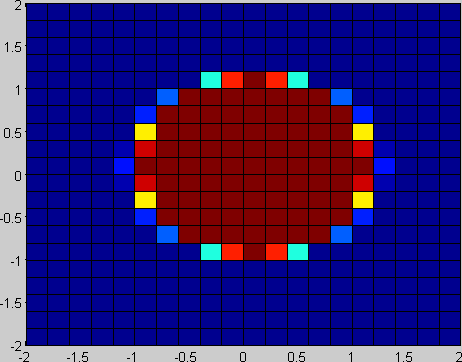
\includegraphics[width=4cm]{filter1.png}}
	\quad
	\subfloat[Bottom near knees]{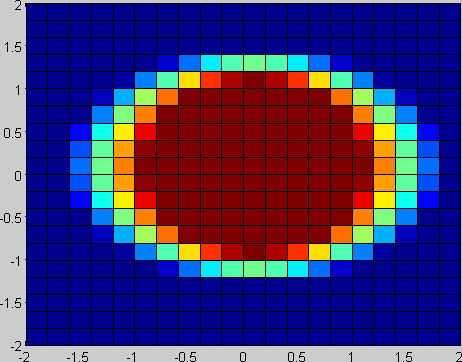
\includegraphics[width=4cm]{filter2.png}}
	\caption{Cross sections through the 3D thigh-filter.  Red = 1, Blue = 0.}
	\label{ThighFilterCrossSections}
\end{figure}

\bigskip
\noindent The 3D filter is 20x20x20 pixels in volume and generated by a simple Matlab function (see \ref{ThighFilter.m}).
It is exported to a custom binary file format and later loaded by the C code where it is stretched to match the dimensions of the thigh.
Two 2D cross-sections of the filter are shown in Figure \ref{ThighFilterCrossSections}.
From these it can be seen that the filter has a cylindrical core of value 1 to match the solid central section of the thigh.
Additional rings of pixels with lower values are built up around the edge of this cylinder towards the bottom.
The idea is that the filter will then fit ``better'' when it is placed exactly in the center if the thigh,
as this is where the filter pixels with the highest values will correspond to filled voxels in the thigh.

The rings are smaller towards the top of the filter so as not to match the area of filled voxels where the thighs join the hips.

\bigskip
\noindent One of the reasons that this cross-correlation approach was attempted first is that it lends itself very nicely to implementation on a stream processor.
The same matrix multiplications and floating point operations can be performed on a large amount of data at once, with no dependencies or iterative behaviour.
Figure \ref{CrossCorrelation} shows how this is implemented using the OpenGL graphics pipeline.
The fragment shader used is listed in \ref{correlation.cg}.

\begin{figure}[tb]
	\vspace{-10pt}
	\centering
	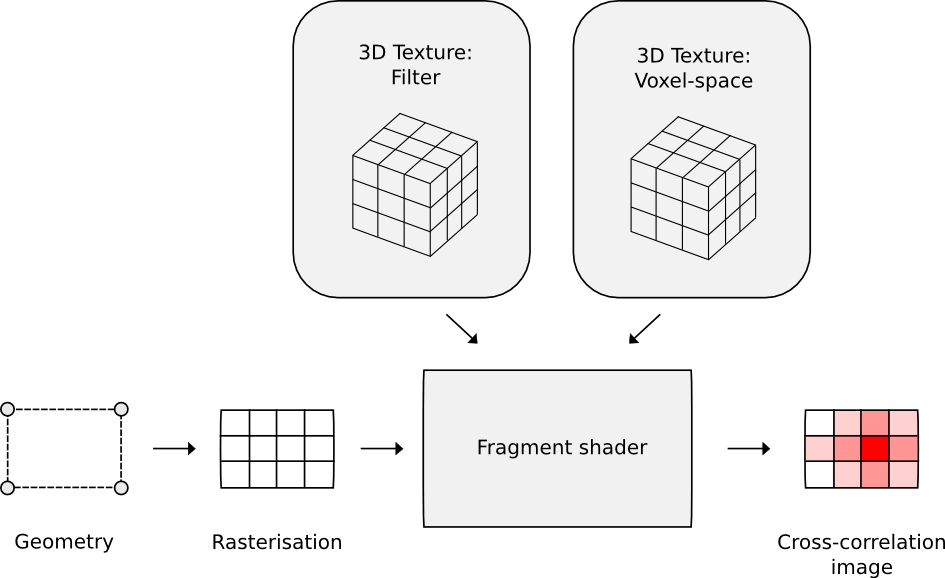
\includegraphics[height=6cm]{correlation.png}
	\caption{How the OpenGL graphics pipeline can be used to accelerate cross-correlation.
		A quad is drawn and rasterised to match the desired size of the cross-correlation image.
		A fragment program is run on each of the generated fragments to evaulate Equation \ref{eqn:CrossCorrelation}.}
	\label{CrossCorrelation}
\end{figure}

The implementation creates an additional matrix $\mathbf{M}_2$ that is used to convert between the coordinate spaces of OpenGL textures to that of our filters and voxel-space.
It also contains a translate and a scale operation to align the filter with the hips, and scale it to the right size.
The values used in these transformations are obtained from Section \ref{LocatingCenter}.
Our original $\mathbf{M}$ from Equation \ref{eqn:Matrix} is applied to $\mathbf{M}_2$ like so:

\begin{equation}
	\mathbf{M} = \mathbf{M} * \mathbf{M}_2
\end{equation}

\bigskip
\noindent The results from this method reveal that perhaps this kind of simple correlation is not suitable for detecting parts of the body in our sample data.
Figure \ref{ParameterSpace} shows the cross-correlation image for a thigh that is oriented straight, in standing position.
It can be seen that $\theta$ is generally correct - horizontally, the concentration of intensity is in the middle of the image, meaning $\theta \simeq 0$.
However vertically there is a far greater concentration of color towards the bottom of the image where $\alpha$ is positive.
This is because here the thigh-filter has been rotated inwards towards the center of the figure, and is matching parts of both left and right legs.

\begin{figure}[tb]
	\vspace{-10pt}
	\centering
	\includegraphics[height=4cm]{parmeterspace.png}
	\caption{An output cross-correlation image, with correlation strength rendered into the red color channel.
		$\theta$ is mapped to the X axis, and $\alpha$ to Y.
		The center of the image is $(\theta, \alpha) = (0,0)$.}
	\label{ParameterSpace}
\end{figure}

A workaround for this is to fix $\alpha = 0$ and only concern ourselves with $\theta$.
This is acceptable, as the movement of the leg along the walking direction is much greater than its movement perpendicular to that direction.
The results from this method are promising, and demonstrate that the algorithm does work to a certain degree.
Techniques for improving the results are presented in section \ref{ImprovedCC}.


\subsection{Active contours}

Active contours are a useful tool in image processing as they allow a shape to be extracted from potentially noisy data.
It is reasoned that active contours could be used to locate the thigh in a noisy 3D voxel-space reconstruction.
An estimation of the likely position of the thigh is first formed by looking for a concentration of voxels below the hip
(see \ref{LocatingCenter}) and either to the left or right side depending which leg is being located.
Cross-sections of the leg are taken at various heights up the leg, centered around this concentration of voxels - see figure \ref{CrossSections}.
An active contour (or snake) is then placed in the middle of each cross-section and allowed to grow to fill the space available.

\begin{figure}[tb]
	\vspace{-10pt}
	\centering
	\subfloat[Lower legs]{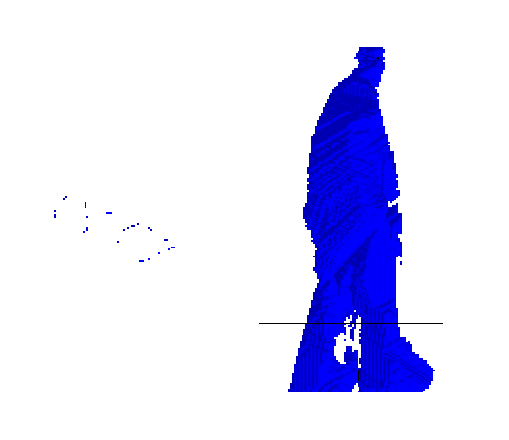
\includegraphics[width=4cm]{crosssections1.png}}
	\quad
	\subfloat[Thigh joining hips]{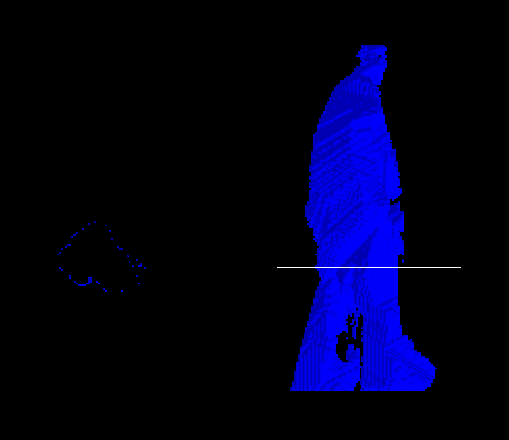
\includegraphics[width=4cm]{crosssections2.png}}
	\caption{Cross sections taken through the legs at various points (after edge-detection.)}
	\label{CrossSections}
\end{figure}

Hopefully each contour will match the interior area of the thigh at its corresponding height up the leg.
The centers of these contours can then be joined together by a straight line to form the center of the model's cylinder.

As described in section \ref{ContourBackground} an active contour is driven by internal energies and external energies.
A trial-and-error approach was used to generate these energy functions - their effectiveness being tested on a series of artificial images.
The images (see Figure \ref{Contours}) were designed to emulate expected cross-sections of thighs at various heights - ranging from elongated areas
near the hips to closed circular areas further down.
An ideal set of energy functions would cause the contour to match the entire of the closed-area images, but not spread out into
the pelvic area when tested on a cross-section of the joint with the hips.

\begin{figure}[tb]
	\vspace{-10pt}
	\centering
	\subfloat[Inside of thigh]{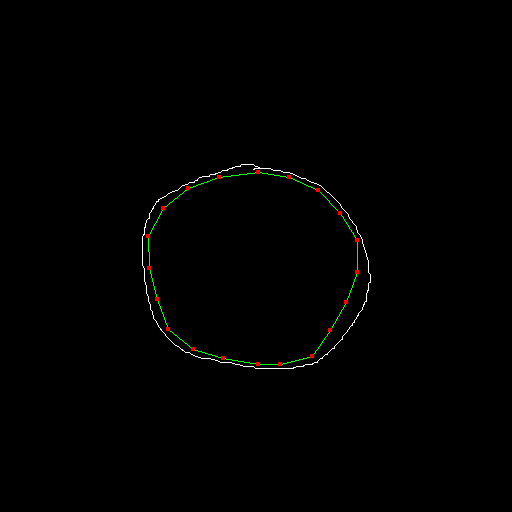
\includegraphics[width=4cm]{contour2.png}}
	\quad
	\subfloat[Thigh joining hips]{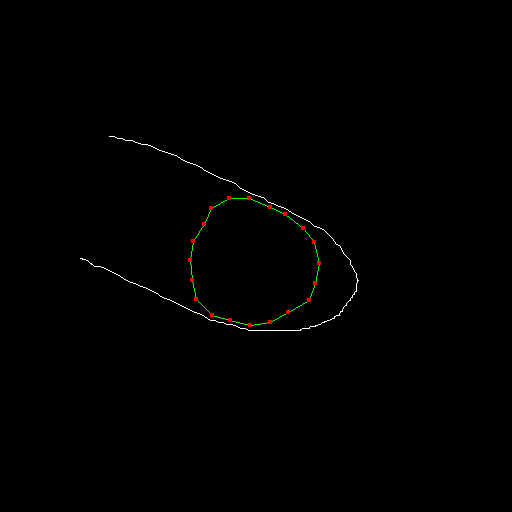
\includegraphics[width=4cm]{contour4.png}}
	\caption{Snakes matching test images for thigh cross-sections.}
	\label{Contours}
\end{figure}

\bigskip
\noindent A set of four energy functions was created.  It should be noted that in the following equations $n$ is the total number of snaxels,
$\mathbf{V}_{i}$ is the position vector of the snaxel at index $i$ around the contour, where $i \in \{1 \cdots n\}$.
Because the contour is closed all subscript arithmetic is modulo $n$, i.e. $\mathbf{V}_{n+1} = \mathbf{V}_{1}$.
Generally $\mathbf{V}_{i}$ is used to denote the old position of the current snaxel, and $\mathbf{V}_{new}$ its proposed new position
currently being evaluated.

\begin{enumerate}
	\item \textbf{Continuity Energy} - designed to maintain an equal spacing between snaxels.
		\begin{equation}
			E_{cont} = \Bigg| \bigg( \frac{1}{n} \sum_{j=1}^n\| \mathbf{V}_{j-1} - \mathbf{V}_{j} \| \bigg) - \bigg( \| \mathbf{V}_{i-1} - \mathbf{V}_{new} \| \bigg) \Bigg|
		\end{equation}
		This function looks at the difference between the average snaxel spacing and the spacing between the new proposed snaxel and its neighbour.
	
	\item \textbf{Balloon energy} - designed to make the snaxels expand outwards to fill an area.
		\begin{equation}
			E_{bal} = \mathbf{n} \cdot (\mathbf{V}_{i} - \mathbf{V}_{new})
		\end{equation}
		Where $\cdot$ is the inner product operator and $\mathbf{n}$ is the normal unit vector of the snaxel away from the origin position $\mathbf{V}_{origin}$:
		\begin{equation}
			n = \frac{\mathbf{V}_{i} - \mathbf{V}_{origin}}{\|\mathbf{V}_{i} - \mathbf{V}_{origin}\|}
		\end{equation}

	\item \textbf{External energy} - stops the snaxels from crossing filled voxels in the image.
		A filled voxel represents the boundary of the area that the contour should describe, and in its simplest form this function is as follows:
		\begin{equation}
			E_{ext} = I(\mathbf{V}_{new})
		\end{equation}
		Where $I(\mathbf{v})$ is the image intensity at the location $\mathbf{v}$.
		
		A problem with this function is that it is not very robust when there is noise present in the image - the area's edge may have gaps and not be a solid filled line.
		To solve this problem we can sample the image intensity in a 7x7 grid around the location being tested:
		\begin{equation}
			E_{ext} = \sum_{x=-3}^3 \sum_{y=-3}^3 I \binom{\mathbf{V}_{new_0} + x}{\mathbf{V}_{new_1} + y}
		\end{equation}
		This second version has the advantage of overcoming problems that occur when the contour is allowed to jump large numbers of pixels at a time -
		it may occasionally skip over a line in the image completely.
	
	\item \textbf{Shape energy} - ensures the contour stays in a circular shape.
		\begin{equation}
			E_{shape} = \Bigg| \bigg( \frac{2}{n}\sum_{j=1}^n \| \mathbf{V}_{j+\frac{n}{2}} - \mathbf{V}_j \| \bigg) - \bigg( \| \mathbf{V}_{i+\frac{n}{2}} - \mathbf{V}_{new} \| \bigg) \Bigg|
		\end{equation}
		This function depends on there being an even number of snaxels in the contour.
		It works by trying to keep the diameters constant (distances between the current snaxel and the one across the shape from it).
		By doing this we can stop the shape becoming elongated.

\end{enumerate}

\noindent The energy function weights were also chosen by trial-and-error.
The weights that were found to work the best were:
\begin{align*}
	w_{cont} &= 1 \\
	w_{ball} &= 0.3 \\
	w_{shape} &= 0.1 \\
	w_{ext} &= 100
\end{align*}

The overall energy function is therefore given by:

\begin{equation}
	E = w_{cont} E_{cont} + w_{ball} E_{ball} + w_{shape} E_{shape} + w_{ext} E_{ext}
\end{equation}

\bigskip
\noindent The implementation in C of the active contour was fairly straightforward.
A \texttt{resetContour} function initialises the contour to a tiny circle at the given location,
and an \texttt{advanceContour} function calculates and updates each snaxel with its next position.
This works by evaluating the energy function at each point in a $k$x$k$ grid centered on the snaxel,
and selecting the one with the lowest value. \cite{SnakeAlgorithm}
The selected point in the grid where the energy function was lowest becomes the snaxel's new position.

This process is repeated until the total change in snaxel position falls below a certain threshold $t$.

Due to its iterative nature it is difficult to find an implementation of this algorithm that is suitable for execution on a stream processor 
However even with a large number of snaxels the C implementation converges on an answer quickly enough for it not to be an issue.

\bigskip
\noindent It is still not certain whether the active contour method is the best way of finding the location of the thigh in an image.
Active contours are generally better suited to locating complex shapes in very noisy greyscale images.
The shape that we are trying to locate here is a simple circle and the values of the pixels in the image are boolean (edge or not-edge).

Perhaps a better approach could be developed by taking some active contour concepts such as internal and external energies,
but restricting the shape to being a perfect circle with a radius $r$ and position $\mathbf{V}$.
This shape would be initialised $r = 0$ and $\mathbf{V} = \mathbf{V}_{origin}$.
Every iteration $r$ would be increased by $1$, and the center $\mathbf{V}$ moved away from any filled pixels inside the circle's area.
Iteration would cease when the radius could be increased no further without filled pixels appearing on both sides.

This approach would allow the circle to expand and center itself inside the leg.
It would stop when it could expand no further without breaching the edge of the shape.
